\documentclass[11pt]{article}
\usepackage{hyperref}
\usepackage{amsmath, amsfonts, amssymb, mathrsfs}
\usepackage{dcolumn}
\usepackage{caption}
\usepackage{subcaption}
\usepackage{filemod}
\usepackage{natbib}
\usepackage[ruled, vlined]{algorithm2e}
\usepackage{floatrow}
\usepackage{setspace}
\usepackage{verbatim}
\usepackage{graphicx}

\hypersetup{
    colorlinks=true,
    linkcolor=blue, 
    urlcolor=black,
    citecolor=blue, 
    }

\oddsidemargin=0.25in
\evensidemargin=0.25in
\textwidth=7in
\textheight=8.75in
\topmargin=-.5in
\addtolength{\oddsidemargin}{-.5in}
\addtolength{\evensidemargin}{-.5in}
\footskip=0.5in
%\doublespacing

\title{Deep Gaussian Processes and Hierarchical Modeling with Functional Data: A Case Study in Cosmological Power Spectra}
\author{Stephen A. Walsh\thanks{Corresponding author: Division of Natural Sciences, 
        Math and Technology, Elms College, {\tt walshst@elms.edu}} \and 
        Annie S. Booth\thanks{Department of Statistics, North Carolina State University} \and
        David Higdon\thanks{Department of Statistics, Virginia Tech} \and
        Marco A.R. Ferreira\footnotemark[3]}
\date{\today}


\begin{document}

\maketitle
\bigskip

\begin{abstract} 
Understanding the structure of our universe and how matter is spread out and expanding is an area of active research. As cosmological surveys grow in complexity, developing surrogate models to efficiently predict matter power spectra is an important research area in cosmology. In this work, we synthesize methods from deep Gaussian processes, Bayesian hierarchical modeling, and basis functions in a novel way to estimate and predict matter power spectra (which are functional in nature) for different cosmologies. Our method has favorable results compared to the benchmark cosmological emulator (Cosmic Emu), and our code is available in a repository.
\end{abstract}

%\vfill

\section{Introduction}
%%%%%%%%%%%%%%%%%%%%%%%%%%%%%%%%%%%%%%%%%%%%%%%%%%%%%%%%%%%%%%%%%%%%%%%%%%%%%%%

To further our understanding of the structure and movement of the universe, researchers utilize numerous cosmological surveys such as the Sloan Digital Sky Survey \citep{york2000sloan} and the upcoming Nancy Grace Roman Space Telescope \citep{Dore2019WFIRST} which are continuously growing in complexity. With these tools, cosmologists aim to continue learning more about cosmic acceleration \citep{caldwell2009physics}. To this end, one important ingredient to aid in this understanding of our universe is the matter power spectrum. 

The matter power spectrum is a fundamental concept in cosmology and describes the distribution of matter as a function of spatial scale. It is often represented as a function of wavenumber $k$ (units Mpc$^{-1}$), which is inversely related to spatial scale. On large scales (i.e., small $k$ values), cosmic expansion dynamics and the matter power spectrum behave according to linear perturbation theory \citep{pietroni2008flowing, lesgourgues2009non}. On smaller scales, non-linear dynamics require the use of computationally intensive simulations; the Coyote Universe \citep{lawrence2010coyote} and more recently the Mira-Titan Universe \citep{moran2023mira} are two simulation suites dedicated to this effort. 

Leveraging these simulations allows for emulation and prediction of the matter power spectrum under varying specifications for eight different cosmological parameters (i.e., different cosmologies). Estimating and understanding the influence of these parameters on cosmic expansion are areas of active research. In addition to presenting the Mira-Titan simulation suite, \cite{moran2023mira} builds off of previous spectrum emulation \citep{lawrence2017mira} to provide the final emulator (Cosmic Emu) based on the full suite of simulations.

\textcolor{blue}{The Cosmic Emu emulator is constructed by (process convolutions, ...). Segue to our method after and compare/contrast with Cosmic Emu.}

Due to the nonstationary behavior expected to be seen in power spectra (e.g., from baryonic acoustic oscillations), we expand on the previous emulation methods and propose a novel synthesis of methods to quantify uncertainty and predict matter power spectra for different cosmologies using deep Gaussian processes (DGPs). In order to handle multiple realizations of functional output (from the Mira-Titan simulation suite), we use hierarchical and basis functions modeling within our DGP framework to accurately estimate and predict power spectra for different cosmologies. When comparing to Cosmic Emu, we see favorable results for our method. The code to reproduce these results are available at \url{https://github.com/stevewalsh124/dgp.hm}. \textcolor{blue}{Please note: this repository is currently private until we hear back regarding permissions for sharing the Mira-Titan data used to train and predict this model.}

The remainder of the paper is organized as follows: Section \ref{sec:data} provides more details regarding the Mira-Titan simulation suite. Section \ref{sec:hm_fit} describes our model and the training procedure for both toy data as well as the Mira-Titan dataset. With this trained model, Section \ref{sec:pred} explains our modeling approach for predictions at held-out cosmologies and compares with other methods. Section \ref{sec:disc} concludes with a discussion of our contributions and avenues for future research.

\section{Data}
\label{sec:data}

The Mira-Titan simulation suite is a dataset consisting of simulated power spectra for 117 different cosmologies. Each of these cosmologies is specified by 8 cosmological parameter values, which we will denote as $\theta \in \mathbb{R}^8$. Different simulation output exists for different values of a ninth value, the redshift; in this work, we fix this value at 0. For each cosmology, we have a set of 18 simulated spectra: an inexpensive spectrum estimated from linear perturbation theory ($y_p$), 16 spectra estimated from lower-resolutions simulations ($y_{\ell_r}, r \in \{1,\dots,16\}$), and one spectrum from a high resolution simulation ($y_h$). 

These spectra are represented as a function of wavenumber $k$, and hence is denoted $P(k)$. Following \cite{moran2023mira}, we model on the emulation space $\mathcal{P}(k)=\log_{10}\left(\frac{k^{1.5}P(k)}{2\pi^2}\right)$. The output is available for $0.001 \leq k \leq 5$ for $n=351$ different values of $k$, but each data type has differing values where it is deemed approximately unbiased. For $k<0.04$, only $y_p$ provides a reliable estimate of the spectra. $y_{\ell_r}$ are valid for $0.04 \leq k \leq 0.25$, and $y_h$ is valid for $0.04 \leq k \leq 5$. Figure \ref{fig:plot_data} shows an example of the output for a particular cosmology.

\begin{figure}[ht]
    \centering
    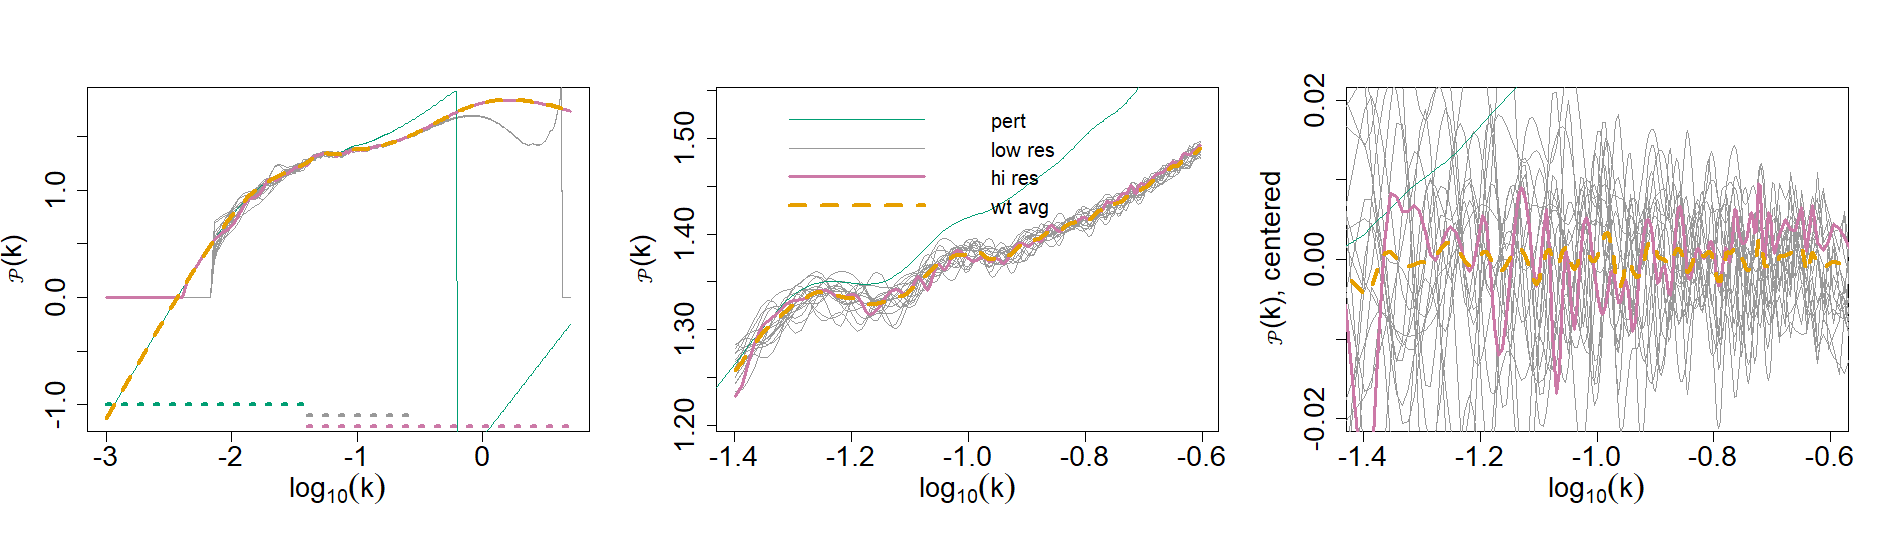
\includegraphics[width=4in]{plot_data.png}
    \caption{The perturbation theory, low resolution runs, and high resolution run for the first training cosmology. The weighted average is also shown as a dashed line. Dotted lines at the bottom indicate where each data type is deemed approximately unbiased.}
    \label{fig:plot_data}
\end{figure}

From the multiple low- and high-resolution spectra across all cosmologies, \cite{moran2023mira} obtain estimates for the precision of these spectra across the $n$ wavenumber values ($p_1,\dots,p_n$) using a log-log regression model, and a multiplier $c$ for the increase in precision from the low- to high- resolution output. Given that the perturbation theory spectra is non-stochastic, we treat this as having a precision of $10^6$. We leverage these precision estimates within our model and calculate a weighted average for each cosmology: $\bar y = AddThisIn$, \textcolor{blue}{where we have four diagonal covariance matrices.}

We will handle the data in two stages.  First, we will focus on 111 training cosmologies and obtain the best esimated spectrum for each.  Second, we will use these estimates to predict the spectra for six held-out cosmologies.

\section{Bayesian Hierarchical Modeling for Particular Cosmologies}
\label{sec:hm_fit}

The main purpose of this section is to describe our first contribution: the use of a Bayesian hierarchical model to estimate the true curve (and provide UQ) for a particular cosmology.  We focus solely on one cosmology, independent of the others.

\subsection{Gaussian Process Model}

Here, we introduce the Bayesian GP model.  We mention the tapering and the formulation of the block covariance matrix.  As well as the posterior conditioning that provides the closed-form solution for the posterior mean and variance.  We can cite Steve's dissertation.

\subsection{Deep Gaussian Process Model}

Here, we expand on the previous section by incorporating a latent layer warping \citep{damianou2013deep}.  We discuss the elliptical slice sampling of $W$, but otherwise it is plugged in to the methods of the previous section with very few changes.

\subsection{Simulation Study}
\label{subsec:sim}

Here, we can provide results from a sim study comparing the GP and DGP, in which case the true curve is known.

\subsection{Estimating Spectra with Mira-Titan Data}
\label{subsec:mira_fit}

Estimate one cosmology with 50,000 runs, and use this as a starting point for each of the others
Here we can provide figures of the predicted mean and variances for a subset of the actual cosmologies.

Images:
\begin{itemize}
    \item Illustration of DGP fit (post mean and UQ, could show cosmicEMU as well?)
    \item estimated warping (or, how all 111 warpings compare)
\end{itemize}


\section{Prediction for Unobserved Cosmologies}
\label{sec:pred}

This section details our second contribution - the use of the Bayesian DGP model of the previous section to predict the curve for held-out cosmologies.

\subsection{PCA-GP Model}
\label{subsec:pca}

Here we describe the PCA-GP model.  We discuss how we use the predicted curves that we got previously as training data.

\begin{itemize}
    \item show breakdown of estimated mean trend, basis functions/PCs, and weights of a particular PC/BF.
\end{itemize}

\subsection{Predicting Spectra from Mira-Titan Data}
\label{subsec:mira_pred}

Here we show results on held-out cosmologies.  We compare to cosmicEMU and Jared's convolution approach. We can also discuss estimation of main effects, interactions amongst the 8 parameters, and variance decomposition.

\begin{itemize}
    \item compare the 4 with boxplot: our DGP training, DGP testing, vs proc conv training (aka Jared's files), proc conv testing (aka Cosmic EMU)
    \item compare the 4's RMSEs as a function of $k$
    \item Main effects
\end{itemize}

\section{Discussion}
\label{sec:disc}

Brief recap, directions for future research: BSS-ANOVA in lieu of DGPs, hydrodynamical sims or TCs as other applications of this methodology. A more detailed sensitivity analysis for the parameters, modeling $W$ across different cosmologies, consider modeling for different redshift values other than $z=0$.

\section{Appendix}
\label{sec:apdx}

The different appendices from dissertation as necessary. Can also put details of dataset in supplementary material.

\bibliographystyle{jasa}
\bibliography{references}

\end{document}
